%\documentclass[11pt,a4paper]{article}
%\usepackage{fullpage}
%\usepackage{beamerarticle}
%\documentclass[handout,xcolor=pdftex,dvipsnames,table]{beamer}
\documentclass[hyperref={unicode=true}]{beamer}
%\documentclass{beamer}

%\usepackage{pgfpages} 
%\pgfpagesuselayout{resize}[a4paper,border shrink=5mm,landscape] 

%%%%%%%%%%%%%%%%%%%%%%%%%%%%%%%%%%%%%%%%%%%%%%%%%%%%%%%%%%%%%%%%%%%%%%%
% КОММЕНТАРИИ
% Нужно ещё взять раздел про поразрядную сортировку из Кнута, в
% частности было бы интересно добавить внешнюю поразрядную
% сортировку. 
%


\usepackage[utf8]{inputenc}
\usepackage[russian]{babel}
\usepackage{../clrscode3e} 
\usepackage[all]{xy}
\usepackage{colortbl}
\usepackage{xcolor}

\definecolor{orange}{cmyk}{0,0.52,1,0}

% \usepackage{beamerthemesplit}

\AtBeginSubsection[]
{
  \begin{frame}<beamer>{Раздел}
    \tableofcontents[currentsection,currentsubsection]
  \end{frame}
}


\newtheorem{rtheorem}{Теорема} 
%default}
%themesplit}

\title{Сортировка за линейное время}
\subtitle{Дискретный анализ 2012/13}
\author{Андрей Калинин, Татьяна Романова}
\date{3 сентября 2012 г. }
\usetheme{default}
%\usefonttheme{serif}
\usefonttheme[onlymath]{serif}
%\usefonttheme{professionalfonts}
%\usetheme{default} 


\begin{document}

\frame{\titlepage}

\frame{
  \frametitle{Прежде чем начать первую лекцию}
  \begin{itemize}
    \item Романова Татьяна Сергеевна, \texttt{tr@umc8.ru}.
    \item Материалы: \texttt{http://k806.ru/daprogram}.
    \item Два семестра, два экзамена. 
    \item В первом семестре 4 лабораторные работы: линейная
      сортировка, словарь, исследование качества программы, поиск подстрок. 
  \end{itemize}
}

\frame{
  \frametitle{Об оценках}
    \begin{columns}
    \begin{column}{0.7 \textwidth}
       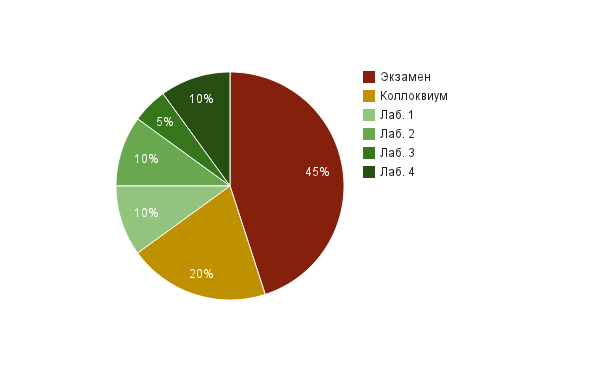
\includegraphics[scale=0.5]{pics/percents.png}
    \end{column}
    \begin{column}{0.3 \textwidth}
       \begin{itemize}
         \item $\geqslant 90 $ --- <<5>> 
         \item $\geqslant 70 $ --- <<4>> 
         \item $\geqslant 60 $ --- <<3>> 
       \end{itemize}
    \end{column}
  \end{columns}
}

\frame{
  \frametitle{Требования к выполнению лабораторных}
    \begin{itemize}
      \item Обязательные (невыполнение снижает оценку до 0):
         \begin{itemize}
            \item cамостоятельная работа;
            \item сдача в указанный срок;
            \item оформление отчета.
         \end{itemize}
       \vspace{1cm}
       \item Желательные (невыполение снижает оценку):
         \begin{itemize}
           \item корректная работа;
           \item оптимальная реализация;
           \item понятный код;
           \item глубокое понимание темы.
         \end{itemize}
    \end{itemize}
}

\frame{
  \frametitle{Литература по курсу}
  \begin{itemize}
  \item Д. Кнут, <<Искусство программирования.>>
  \item Т. Кормен, <<Алгоритмы: построение и анализ.>>
  \item Д. Гасфилд, <<Строки, деревья и последовательности в
    алгоритмах.>>
  \item Witten, <<Managing gigabytes: compressing and indexing
    documents and images.>>
  \item Г. Уоррен, <<Алгоритмические трюки для программистов.>>
  \item \texttt{http://k806.ru/books}
  \end{itemize}
}

%
% Нужно будет ещё добавить требования лабораторным работам
%

%\section[Содержание]{}
\frame{\tableofcontents}

%\section{Литература}
\frame
{
  \frametitle{Литература}

  \begin{itemize}
  \item  Кормен Т., Лейзерсон Ч., Ривест Р., Штайн К.. Алгоритмы:
    построение и анализ, 2-е издание, М.:Вильямс, 2005, стр. 220-239, глава 8,
    <<Сортировка за линейное время>>. 
  \end{itemize}
}

\section{О сортировках и оценках}

\subsection{Оценки}
%\frame{\tableofcontents[currentsubsection]}

\frame
{
  \frametitle{Асимптотичске обозначения}
  \begin{itemize}
    \item $f(n) = O(g(n))$, если существуют константы $c$ и $n_0$ 
          такие, что $0 \leqslant f(n) \leqslant cg(n)$ 
          для всех $n \geqslant n_0$.
    \vspace{1cm}
    \item $f(n) = \Omega(g(n))$, если существуют константы $c$ и $n_0$ 
         такие, что $0 \leqslant cg(n) \leqslant f(n)$ 
          для всех $n \geqslant n_0$.
    \vspace{1cm}
    \item $f(n) = \Theta(g(n))$, если существуют константы $c_1$, $c_2$ и $n_0$
        такие, что $0 \leqslant c_1g(n) \leqslant f(n) \leqslant c_2g(n)$
        для всех $n \geqslant n_0$.
   \end{itemize} 
}

\frame
{
   \frametitle{Линейность}
   \begin{itemize}
    \item $f(n) = O(n)$
    \item $n$ --- размерность задачи.
    \item Линейность (функция $f(n)$): 
    \begin{itemize}
      \item Количество элементарных операций. 
      \item Объём оперативной памяти.  
      \item Могут оцениваться другие параметры: количество процессорных ядер
        или серверов. 
    \end{itemize}
  \end{itemize}
}

\frame{
  \frametitle{Скользкие места}
  \begin{itemize}
  \item Не может быть алгоритма, работающего за $O(n)$ и не укладывающегося в
    $O(n)$ по памяти. 
  \item В строгом смысле элементарные операции ---   выполняемые
    команды машиной Тьюринга (или эквивалентной моделью.)
  \item В практическом смысле элементарность операций определяется
    реальным процессором. 
  \end{itemize}
}

\frame{
  \frametitle{На практике}
  \begin{itemize}
    \item Всегда есть физические ограничения: размер оперативной
      памяти, жёстких дисков. 
    \item Иерархия оперативной памяти: регистры, кэш-память L1, L2,
      DRAM, жёсткие диски, распределённые файловые системы. 
    \item Константа $c$ может быть слишком большой. 
  \end{itemize}
}

\subsection{Сортировки}

\frame{
  \frametitle{Петабайтная сортировка (Google, 2008)}
  \begin{itemize}
  \item Петабайт данных (1024 терабайта, $10^{13}$
      100-байтных записей).
    \item 48 000 жёстких дисков на 4 000 серверах. 
    \item Трёхкратное дублирование записей. 
    \item Работа в течение 6 часов. 
    \item На каждом запуске сортировки как минимум один диск
      выходит из строя. 
    \item Применяемые решения: распределённая файловая система (Google
      FS) и алгоритмы распределения задач (MapReduce).
    \end{itemize}
}

%\frame{
%  \frametitle{Развитие алгоритмов сортировки}
%  \begin{itemize}
%    \item $O(n \log \log n)$.
%    \item Случайные сортировки. 
%    \item Ориентированные на использование кэш-памяти.
%    \item Параллельные и распределённые сортировки. 
%  \end{itemize}
%}

%\frame
%{
%  \frametitle{Что ещё интересного}
%  \begin{itemize}
%    \item Бинарный поиск с учётом кеш-памяти
%  \end{itemize}
%}

\subsection{Нижняя оценка сортировок сравнением}

\frame
{
  \frametitle{Сортировка сравнением}
  \begin{itemize}
  \item Последовательность $\langle a_1, a_2, \ldots, a_n \rangle$.
  \item При сортировке используются только попарные сравнения:
    $a_i < a_j$, $a_i \leq a_j$, $a_i = a_j$, $a_i  \geq a_j$,
    $a_i > a_j$.
  \item Предполагаем, что все элементы различны, тем самым можно
    считать что используется только $a_i \leq a_j$.
  \end{itemize}
}

\frame
{
  \frametitle{Модель дерева решений}
  Дерево решений: 
  \begin{itemize}
    \item Полное бинарное дерево, в котором представлены операции
      сравнения элементов. 
    \item Внутренние узлы помечены меткой $i:j$, $1 \leq i,j \leq n$,
      указывающие на сравнение $a_i$ и $a_j$. 
    \item Лист помечен перестановкой 
      $\langle \pi(1), \pi(2), \ldots, \pi(n) \rangle$, дающее
      окончательное упорядочение элементов  
      $\langle a_{\pi(1)} \leq a_{\pi(2)} \leq \cdots \leq
      a_{\pi(n)}\rangle$.
    \item Корректность сортировки сравнением: соответствующее дерево
      решений должно содержать все $n!$ перестановок исходных $n$
      элементов, к которым можно проложить путь реального выполнения
      сортировки (<<достижимые>> листья.)
  \end{itemize}
}

\frame
{
  \frametitle{Сортировка вставкой трёх элементов}
$\langle a_1 = 6, a_2 = 8, a_3 = 5 \rangle $
\[\xygraph{
  [] *+[o]+[F]{1:2}
  (-@{=}_\leq[dll] *+=[o]+[F]{2:3}
    (-_\leq[dl] *+[F]{\langle 1,2,3 \rangle}
    ,-@{=}^{>}[dr] *+=[o]+[F]{1:3}
      (-_\leq[dl] *+[F]{\langle 1,3,2 \rangle }
      ,-@{=}^{>}[dr] *+[F]{\langle 3,1,2 \rangle }
      )
    )
  ,-^{>}[drr] *+=[o]+[F]{1:3}
    (-_\leq[dl] *+[F]{\langle 2,1,3 \rangle}
    ,-^{>}[dr] *+=[o]+[F]{2:3}
      (-_\leq[dl] *+[F]{\langle 2,3,1 \rangle }
      ,-^{>}[dr] *+[F]{\langle 3,2,1 \rangle }
      )
    )
  )
}
\]
}

\frame
{
  \frametitle{Нижняя оценка для наихудшего случая}
  \begin{rtheorem}
    В наихудшем случае в ходе выполнения любого алгоритма сортировки
    сравнением выполняется $\Omega(n\log_2 n)$ сравнений. 
  \end{rtheorem}
  \begin{proof}
    Для дерева решений сортировки $n$ элементов и высотой $h$ c $l$ достижимыми листьями:
    \[
    n! \leq l \leq 2^h\Rightarrow h \geq \log_2(n!) = \Omega(n\log_2n)
    \]
  \end{proof}
}


\section{Алгоритмы}

\subsection{Сортировка подсчётом}

\frame
{
  \frametitle{Общая идея}
  \begin{itemize}
    \item $\langle a_1, \ldots, a_n\rangle$, 
      $a_i$ --- целое и $0 \leq a_i \leq k$.
    \item Если $k = O(n)$ то время работы равно $\Theta(n)$
    \item Для каждого $a_i$ определяется $c_i = \left|\{a_k | a_k <
      a_i\}\right|$.
    \item $c_i$ определяет местоположение $a_i$ в отсортированной
      последовательности. 
  \end{itemize}
}

\frame
{
  \frametitle{Алгоритм}
\begin{codebox} 
\Procname{$\proc{Counting-Sort}(A)$} 
\li \For $i \gets 0$ \To $k$ 
\li    \Do $C[i] \gets 0$ \End
\li \For $j \gets 1$ \To $\id{length}[A]$
\li   \Do $C[A[j]] \gets C[A[j]]+1$ \End
\li \Comment В $C[i]$ хранится количество элементов, равных $i$.
\li \For $i \gets 1$ \To $k$
\li    \Do $C[i] \gets C[i]+C[i-1]$ \End
\li \Comment В $C[i]$ --- количество элементов, не превышающих $i$.
\li \For $j \gets \id{length}[A]$ \Downto 1
\li \Do $B[C[A[j]]]  \gets A[j]$
\li $C[A[j]] \gets C[A[j]] - 1$
\End 
\end{codebox} 

}

\frame
{
  \frametitle{Пример}
  \begin{tabular}{cl}
    $A$    & \begin{tabular}{|c|c|c|c|c|c|c|c|}\hline 2 & 5 & 3 & 0 &
      2 & 3 & 0 & 3\\ \hline\end{tabular}, $0 \leq a_i \leq 5$\\
 & \\
    $C$    & \begin{tabular}{|c|c|c|c|c|c|}\hline 2 & 0 & 2 & 3 & 0 &
      1 \\ \hline\end{tabular} $\rightarrow$
    \begin{tabular}{|c|c|c|c|c|c|}\hline 2 & 2 & 4 & 7 & 7 & 8 \\
      \hline\end{tabular}
  \end{tabular}

  \begin{tabular}{cc}
    $B$ & $C$ \\
   \begin{tabular}{|c|c|c|c|c|c|c|c|}
      \hline ~ & ~ & ~ & ~ & ~ & ~ & 3 & ~ \\
      \hline ~ & 0 & ~ & ~ & ~ & ~ & 3 & ~ \\
      \hline ~ & 0 & ~ & ~ & ~ & 3 & 3 & ~ \\
      \hline ~ & 0 & ~ & 2 & ~ & 3 & 3 & ~ \\
      \hline 0 & 0 & ~ & 2 & ~ & 3 & 3 & ~ \\
      \hline 0 & 0 & ~ & 2 & 3 & 3 & 3 & ~ \\
      \hline 0 & 0 & ~ & 2 & 3 & 3 & 3 & 5 \\
      \hline 0 & 0 & 2 & 2 & 3 & 3 & 3 & 5 \\
      \hline
    \end{tabular} &
   
    \begin{tabular}{|c|c|c|c|c|c|}
      \hline 2 & 2 & 4 & \cellcolor{orange}\textbf{6} & 7 & 8 \\
      \hline \cellcolor{orange}\textbf{1} & 2 & 4 & 6 & 7 & 8 \\
      \hline 1 & 2 & 4 & \cellcolor{orange}\textbf{5} & 7 & 8 \\
      \hline 1 & 2 & \cellcolor{orange}\textbf{3} & 5 & 7 & 8 \\
      \hline \cellcolor{orange}\textbf{0} & 2 & 3 & 4 & 7 & 8 \\
      \hline 0 & 2 & 3 & \cellcolor{orange}\textbf{3} & 7 & 8 \\
      \hline 0 & 2 & 3 & 3 & 7 & \cellcolor{orange}\textbf{7} \\
      \hline 0 & 2 & \cellcolor{orange}\textbf{2} & 3 & 7 & 7 \\
      \hline
    \end{tabular}
\end{tabular}

}

\frame
{
  \frametitle{Свойства сортировки подсчётом}
  \begin{itemize}
    \item Не является сортировкой сравнением: ни одна пара элементов
      не сравнивается друг с другом. 
    \item Линейная (вернее, $\Theta(k+n)$, но при $k=O(n)$ время
      выполнения $\Theta(n)$).
    \item Устойчивая (стабильная.) 
    \item Требует дополнительную память под массивы $C$ и $B$ размером $n$. 
  \end{itemize}
}


\subsection{Поразрядная сортировка}
\frame
{
  \frametitle{Общая идея}
  \begin{itemize}
    \item $d$-значные числа последовательно сортируются по разрядам: от младшего к
      старшему. 
    \item При использовании устойчивой сортировки --- корректное
      упорядочивание. 
    \item Если внутренняя сортировка линейная, то и поразрядная
      сортировка тоже линейная.
  \end{itemize}
}
\frame
{
%\newcolumntype{K}{\columncolor{orange}\raggedright}
  \frametitle{Пример}
  \begin{tabular}{|c@{}c@{}c|}
    \hline
    3 & 2 & 9 \\
    4 & 5 & 7 \\
    6 & 5 & 7 \\
    8 & 3 & 9 \\
    4 & 3 & 6 \\
    7 & 2 & 0 \\
    3 & 5 & 5 \\
    \hline
  \end{tabular}\uncover<2->{~$\Rightarrow$
  \begin{tabular}{|cc>{\columncolor{orange}}c|}
    \hline
    7 & 2 & 0 \\
    3 & 5 & 5 \\
    4 & 3 & 6 \\
    4 & 5 & 7 \\
    6 & 5 & 7 \\
    3 & 2 & 9 \\
    8 & 3 & 9 \\
    \hline
  \end{tabular}}\uncover<3->{~$\Rightarrow$
  \begin{tabular}{|c>{\columncolor{orange}}cc|}
    \hline
    7 & 2 & 0 \\
    3 & 2 & 9 \\
    4 & 3 & 6 \\
    8 & 3 & 9 \\
    3 & 5 & 5 \\
    4 & 5 & 7 \\
    6 & 5 & 7 \\
    \hline
  \end{tabular}}\uncover<4->{~$\Rightarrow$
  \begin{tabular}{|>{\columncolor{orange}}ccc|}
    \hline
    3 & 2 & 9 \\
    3 & 5 & 5 \\
    4 & 3 & 6 \\
    4 & 5 & 7 \\
    6 & 5 & 7 \\
    7 & 2 & 0 \\
    8 & 3 & 9 \\
    \hline
  \end{tabular}}
}
\frame
{
  \frametitle{Алгоритм}
  \begin{codebox}
    \Procname{$\proc{Radix-Sort}(A, d)$}
      \li \For $i \gets 1$ \To $d$
      \li \Do Устойчивая сортировка массива $A$ по $i$-ой цифре
  \end{codebox}
  \begin{rtheorem}
    Для $n$ $d$-значных чисел, в которых каждая цифра принимает одно
    из $k$ значений, алгоритм $\proc{Radix-Sort}$ позволяет выполнить
    корректную сортировку за время $\Theta(d(n+k))$, если внутренняя
    устойчивая сортировка имеет время работы $\Theta(n+k)$.
  \end{rtheorem}
}

\frame{
  \frametitle{Какие цифры выбрать?}
  \begin{rtheorem}
    Для $n$ $b$-битовых чисел и натурального числа $r \leq b$ (цифры
    из $r$ битов) алгоритм
    $\proc{Radix-Sort}$ выполнит сортировку за время $\Theta\left(\dfrac{b}{r}(n+2^r)\right)$.
  \end{rtheorem}
~\\
~\\
~\\
\uncover<2->{
  Тем самым: 
  \begin{itemize}
  \item Для $b < \lfloor \log_2(n) \rfloor$ асимптотически оптимален
    выбор $r=b$.
    \item А для $b \geq \lfloor \log_2(n) \rfloor$: $r=\lfloor
      \log_2(n) \rfloor$
  \end{itemize}
}
}

\frame{
  \frametitle{Свойства поразрядной сортировки}
  \begin{itemize}
    \item Линейная, устойчивая, требуется дополнительная память (из-за
      сортировки подсчётом.) 
    \item Может понадобиться много проходов. 
    \item Несмотря на асимптотическую линейность, для конкретных
      значений $n$ и $r$ сортировки сравнением могут быть
      предпочтительнее из-за разных значений постоянных множителей. 
  \end{itemize}
}

\subsection{Карманная сортировка}
\frame
{
  \frametitle{Общая идея}
  \begin{itemize}
    \item На вход поступают $n$ вещественных чисел, порождённых случайным процессом и
      равномерно распределённых в интервале $[0,1)$.
    \item $[0,1)$ разбивается на $n$ одинаковых интервалов
      (<<карманов>>, buckets)
    \item Числа помещаются в список, соответствующий каждому
      карману. Т.к. распределене равномерное, в одном кармане
      появляется не очень много чисел. 
    \item Все списки сортируются (вставкой.)
    \item Результат получается объединением (один проход по всем спискам.)
  \end{itemize}
}
\frame
{
  \frametitle{Алгоритм}
  \begin{codebox}
    \Procname{$\proc{Bucket-Sort}(A)$}
    \li $n \gets \id{length}[A]$
    \li \For $i \gets 1$ \To $n$
    \li  \Do Вставить элемент $A[i]$ в список 
    $B\left[\lfloor nA[i]\rfloor\right]$ \End
    \li \For $i \gets 0$ \To $n-1$
    \li   \Do Сортировка вставкой списка $B[i]$ \End
    \li Объединение списков $B[0], B[1], \ldots, B[n-1]$
  \end{codebox}


}
\frame
{
  \frametitle{Пример}
  \begin{center}
  \begin{tabular}{r|c|cr|l|}
    \multicolumn{2}{r}{$A$} & \multicolumn{3}{c}{$B$} \\
    \cline{2-2}\cline{5-5}
    1 & .78 & ~ & 0 & $\emptyset$\\
    \cline{2-2}\cline{5-5}
    2 & .17 & & 1 & $\langle .12, .17 \rangle$\\
    \cline{2-2}\cline{5-5}
    3 & .39 & & 2 & $\langle .21, .23, .26 \rangle $\\
    \cline{2-2}\cline{5-5}
    4 & .26 & & 3 & $\langle .39 \rangle$\\
    \cline{2-2}\cline{5-5}
    5 & .72 & & 4 & $\emptyset$\\
    \cline{2-2}\cline{5-5}
    6 & .94 & & 5 & $ \emptyset$\\
    \cline{2-2}\cline{5-5}
    7 & .21 & & 6& $\langle .68 \rangle$\\
    \cline{2-2}\cline{5-5}
    8 & .12 & & 7& $\langle .72, .78 \rangle$\\
    \cline{2-2}\cline{5-5}
    9 & .23 & & 8& $\emptyset $\\
    \cline{2-2}\cline{5-5}
    10 & .68 & & 9 & $\langle .94 \rangle$\\
    \cline{2-2}\cline{5-5}
  \end{tabular}
  \end{center}

}
\frame
{
  \frametitle{Линейность}
  $n_i$ --- количество элементов в кармане $B[i]$. Тогда время работы алгоритма:
  \[
  T(n) = \Theta(n) + \sum_{i=0}^{n-1}O(n_i^2) \Rightarrow
  E[T(n)] = \Theta(n) + \sum_{i=0}^{n-1}O(E[n_i^2])
  \]
  Для всех $i=0, 1, \ldots, n-1$:
  \[
  E[n_i^2] = 2 - \frac{1}{n} \Rightarrow T(n) = \Theta(n)+n\cdot
  O\left(2-\frac{1}{n}\right) = \Theta(n)
  \]
}
\frame
{
  \frametitle{Количество элементов в одном кармане}
  \[
  \begin{split}
  X_{ij} &= I\{A[j]\in B[i]\} \Rightarrow n_i = \sum_{j=1}^nX_{ij},    \\
  E[n_i^2] &=\sum_{j=1}^nE[X_{ij}^2] + \sum_{1 \leq j \leq
    n}\sum_{\substack{1\leq k \leq n \\  k \neq j}}E[X_{ij}X_{ik}], \\
  E[X_{ij}^2] &=
  1\cdot\frac{1}{n}+0\cdot\left(1-\frac{1}{n}\right)=\frac{1}{n}, \\
  E[X_{ij}X_{ik}] &= E[X_{ij}]E[X_{ik}] =
  \frac{1}{n}\cdot\frac{1}{n}=\frac{1}{n^2}, \\
  E[n_i^2] &= n\cdot\dfrac{1}{n} + n(n-1)\cdot \dfrac{1}{n^2}=1+
  \dfrac{n-1}{n}= 2 - \dfrac{1}{n}.
  \end{split}
  \]
}

\end{document}
    
